\documentclass[format=acmsmall, review=false, screen=true]{acmart}

\usepackage{booktabs} % For formal tables

% Metadata Information
\acmJournal{CSCW}
\acmVolume{X}
\acmNumber{X}
\acmArticle{XX}
\acmYear{2018}
\acmMonth{4}
\copyrightyear{2018}
%\acmArticleSeq{9}

% Copyright
%\setcopyright{acmcopyright}
\setcopyright{acmlicensed}
%\setcopyright{rightsretained}
%\setcopyright{usgov}
%\setcopyright{usgovmixed}
%\setcopyright{cagov}
%\setcopyright{cagovmixed}

% DOI
\acmDOI{0000001.0000001}

% Paper history
\received{April 2018}
\received[revised]{July 2018}
%\received[accepted]{June 2009}


\usepackage[ruled]{algorithm2e} % For algorithms
\renewcommand{\algorithmcfname}{ALGORITHM}
\SetAlFnt{\small}
\SetAlCapFnt{\small}
\SetAlCapNameFnt{\small}
\SetAlCapHSkip{0pt}
\IncMargin{-\parindent}
% Arabic page numbers for submission.  Remove this line to eliminate
% page numbers for the camera ready copy
% \pagenumbering{arabic}

% Load basic packages
\usepackage{balance}       % to better equalize the last page
\usepackage{graphics}      % for EPS, load graphicx instead
\usepackage{todonotes}     % for \todo
%\usepackage[T1]{fontenc}   % for umlauts and other diaeresis
%\usepackage{txfonts}
%\usepackage{mathptmx}
%\usepackage[pdflang={en-US},pdftex]{hyperref}
%\usepackage{color}
\usepackage{booktabs}
\usepackage{subcaption}
\usepackage{textcomp}
\PassOptionsToPackage{warn}{textcomp}
%\usepackage[table]{xcolor}

% Some optional stuff you might like/need.
\usepackage{microtype}        % Improved Tracking and Kerning
% \usepackage[all]{hypcap}    % Fixes bug in hyperref caption linking
% \usepackage{ccicons}          % Cite your images correctly!
% \usepackage[utf8]{inputenc} % for a UTF8 editor only

% If you want to use todo notes, marginpars etc. during creation of
% your draft document, you have to enable the "chi_draft" option for
% the document class. To do this, change the very first line to:
% "\documentclass[chi_draft]{sigchi}". You can then place todo notes
% by using the "\todo{...}"  command. Make sure to disable the draft
% option again before submitting your final document.
%\usepackage{todonotes}

% Paper metadata (use plain text, for PDF inclusion and later
% re-using, if desired).  Use \emtpyauthor when submitting for review
% so you remain anonymous.


\newcommand{\FIXME}[1]{\textcolor{red}{[\textbf{FIXME}: \textit{#1}]}}
\newcommand{\TODO}[1]{\textcolor{red}{[\textbf{FIXME}: \textit{#1}]}}

\newcommand\leadin[1]{%
    \vskip 5pt \noindent\textbf{#1.} %
}
\newcommand\leadinx[1]{%
    \vskip 5pt \noindent\textbf{#1} %
}

%
%\def\sharedaffiliation{%
%\end{tabular}
%\begin{tabular}{c}}
%

\clubpenalty=10000
\widowpenalty=10000

% llt: Define a global style for URLs, rather that the default one
%\makeatletter
%\def\url@leostyle{%
%  \@ifundefined{selectfont}{
%    \def\UrlFont{\sf}
%  }{
%    \def\UrlFont{\small\bf\ttfamily}
%  }}
%\makeatother
%\urlstyle{leo}

% To make various LaTeX processors do the right thing with page size.
%\def\pprw{8.5in}
%\def\pprh{11in}
%\special{papersize=\pprw,\pprh}
%\setlength{\paperwidth}{\pprw}
%\setlength{\paperheight}{\pprh}
%\setlength{\pdfpagewidth}{\pprw}
%\setlength{\pdfpageheight}{\pprh}

% Make sure hyperref comes last of your loaded packages, to give it a
% fighting chance of not being over-written, since its job is to
% redefine many LaTeX commands.
% \definecolor{linkColor}{RGB}{6,125,233}

% create a shortcut to typeset table headings
% \newcommand\tabhead[1]{\small\textbf{#1}}


% Document starts
\begin{document}

% Title portion. Note the short title for running heads
\title[ORES]{ORES: Facilitating re-mediation of Wikipedia's socio-technical problems}

\author{Redacted F. Review}
\orcid{1234-5678-9012-3456}
\affiliation{%
  \institution{XXXXXXX}
  \streetaddress{XXXXXXX}
  \city{XXXXX}
  \state{XX}
  \postcode{12345}
  \country{XXX}}
\email{XXXX@XX.XX}

\author{Redacted G. Review}
\orcid{1234-5678-9012-3456}
\affiliation{%
  \institution{XXXXXXX}
  \streetaddress{XXXXXXX}
  \city{XXXXX}
  \state{XX}
  \postcode{12345}
  \country{XXX}}
\email{XXXX@XX.XX}

\renewcommand{\shortauthors}{XXX et al.}


\begin{abstract}
Algorithmic systems---from rule-based bots to machine learning classifiers---have a long history of supporting the essential work of content moderation and other curation work in peer production projects.  From counter-vandalism to task routing, basic machine prediction has allowed open knowledge projects like Wikipedia to scale to the largest encyclopedia in the world, while maintaining quality and consistency.  However, conversations about how quality control should work and what role algorithms should play have generally been led by the expert engineers who have the skills and resources to develop and modify these complex algorithmic systems. In this paper, we describe ORES: an algorithmic scoring service that supports real-time scoring of wiki edits using multiple independent classifiers trained on different datasets. ORES decouples several activities that have typically all been performed by engineers: choosing or curating training data, building models to serve predictions, auditing predictions, and developing interfaces or automated agents that act on those predictions. This meta-algorithmic system was designed to open up socio-technical conversations about algorithmic systems in Wikipedia to a broader set of participants.  In this paper, we discuss the theoretical mechanisms of social change ORES enables and detail case studies in participatory machine learning around ORES from the 4 years since its deployment.

\end{abstract}


%
% The code below should be generated by the tool at
% http://dl.acm.org/ccs.cfm
% Please copy and paste the code instead of the example below.
%
\begin{CCSXML}
<ccs2012>
<concept>
<concept_id>10003033.10003106.10003114.10011730</concept_id>
<concept_desc>Networks~Online social networks</concept_desc>
<concept_significance>500</concept_significance>
</concept>
<concept>
<concept_id>10010147.10010257.10010258.10010259.10010263</concept_id>
<concept_desc>Computing methodologies~Supervised learning by classification</concept_desc>
<concept_significance>500</concept_significance>
</concept>
<concept>
<concept_id>10010405.10010455.10010461</concept_id>
<concept_desc>Applied computing~Sociology</concept_desc>
<concept_significance>500</concept_significance>
</concept>
<concept>
<concept_id>10011007.10011074.10011075.10011079.10011080</concept_id>
<concept_desc>Software and its engineering~Software design techniques</concept_desc>
<concept_significance>500</concept_significance>
</concept>
<concept>
<concept_id>10010520.10010521.10010537.10003100</concept_id>
<concept_desc>Computer systems organization~Cloud computing</concept_desc>
<concept_significance>100</concept_significance>
</concept>
</ccs2012>
\end{CCSXML}


\ccsdesc[500]{Networks~Online social networks}
\ccsdesc[500]{Computing methodologies~Supervised learning by classification}
\ccsdesc[500]{Applied computing~Sociology}
\ccsdesc[500]{Software and its engineering~Software design techniques}
\ccsdesc[100]{Computer systems organization~Cloud computing}

%
% End generated code
%


\keywords{Wikipedia, Reflection, Systems, Machine learning, Transparency, Fairness, Successor, Margin, Algorithms, Governance, Articulation}

\maketitle

\section{Introduction}
\label{sec:introduction}
Wikipedia -- the free encyclopedia that anyone can edit -- faces many challenges in maintaining the quality of its articles and sustaining the volunteer community of editors. The people behind the hundreds of different language versions of Wikipedia have long relied on automation, bots, expert systems, recommender systems, human-in-the-loop assisted tools, and machine learning to help moderate and manage content at massive scales. The issues around artificial intelligence in Wikipedia are as complex as those facing other large-scale user-generated content platforms like Facebook, Twitter, or YouTube, as well as traditional corporate and governmental organizations that must make and manage decisions at scale. And like in those organizations, Wikipedia's automated classifiers are raising new and old issues about truth, power, responsibility, openness, and representation.

Yet Wikipedia's approach to AI has long been different than in the corporate or governmental contexts typically discussed in emerging fields like Fairness, Accountability, and Transparency in Machine Learning (FATML) or Critical Algorithms Studies (CAS). The volunteer community of editors has strong ideological principles of openness, decentralization, and consensus-based decision-making. The paid staff at the non-profit Wikimedia Foundation---which legally owns and operates the servers---are not tasked with making editorial decisions about content\footnote{Except in rare cases, such as content that violates U.S. law, see http://enwp.org/WP:OFFICE}. This is instead the responsibility of the volunteer community, where a self-selected set of developers build tools, bots, and advance technologies in broad consultation with the community. Even though Wikipedia's longstanding socio-technical system of algorithmic governance is far more open, transparent, and accountable than most platforms operating at Wikipedia's scale, ORES, the system we present in this paper, pushes even further on the crucial issue of who is able to participate in the development and use of advance technologies.

ORES represents several innovations in openness in machine learning, particularly in seeing openness as a socio-technical challenge that is as much about scaffolding support as it is about open-sourcing code and data. With ORES, volunteers can curate labeled training data from a variety of sources for a particular purpose, commission the production of a machine classifier based on particular approaches and parameters, and make this classifier available via an API which anyone can query to score any edit to a page -- operating in real time on the Wikimedia Foundation's servers. Currently, 78 classifiers have been produced for 37 languages, classifying edits in real time on criteria like ``damaging / not damaging'', ``good faith / bad faith'', or an ordinal quality scale. ORES intentionally does not seek to produce a single classifier to enforce a gold standard of quality, nor does it prescribe particular ways in which scores and classifications will be incorporated into fully automated bots and semi-automated editing interfaces. Instead, ORES was built as a kind of cultural probe to support an open-ended set of community efforts to reimagine what machine learning in Wikipedia is and who it is for.

\subsection{Audiences for this work}
The issue of open participation in machine learning raises many issues that are widely relevant to both researchers of peer production platforms like Wikipedia, as well as those working across CSCW, social computing, machine learning, and critical algorithms studies.

To researchers of CSCW systems, this paper discusses the design and role of a technical system that supports a novel type of collaborative meta-work, as ORES makes it possible for volunteers commission the production of machine learning classifiers that other editors can use to support a variety of collaborative work practices in an established community of practice. In this paper, we detail this system's design as it was built to align with the particular ways in which volunteers work in Wikipedia. We also describe how ORES has altered the meta-work of Wikimedia tool developers.

To the FATML/CAS communities, we are introducing an open-by-design advanced algorithmic platform that is widely used to maintain a critical information resource.  This platform and its context implement several of the dominant recommendations for algorithmic system builders around transparency and community consent.  Through the deployment of this system and subsequent design iterations, we are able to discuss novel practical considerations for what openness, accountability, and transparency mean in a large scale, real world system.

To algorithmic system-builders, we describe how we have approached key issues in developing a working, scalable, and robust system that matches the decentralized work practices of end-users in Wikipedia.  Some of these approaches apply well described techniques (e.g. distributed processing and caching) while are novel strategies for giving tool developers and their users flexibility over how to use ORES's algorithmic predictions (e.g. model interrogation and threshold optimization).

At one level, ORES is widely relevant to researchers across social computing platforms, but it has specific relevance for researchers of commons-based peer production platforms like Wikipedia. ORES was created in the context of Wikipedia's much-discussed issues around newcomer socialization and inclusion. Wikipedia's existing algorithmic infrastructure for supporting various kinds of decision-making has generally been built by volunteers focused on quality control -- removing spam, hate speech, vandalism, and low-quality content as soon as possible. Newcomer socialization has suffered from an apparent tradeoff as Wikipedians focused heavily on efficient quality management strategies\cite{halfaker2013rise, halfaker2014snuggle}. Peer production projects generally appear to struggle with balancing managing quality and participation\cite{teblunthuis2018revisiting}, and automation in Wikipedia has generally made it more difficult for newcomers.

Past work has attempted to directly intervene by making tools\cite{halfaker2014snuggle} and designing spaces\cite{morgan2013tea} that directly support newcomer socialization.  While some of these interventions have shown promise\cite{morgan2018evaluating}, technological hurdles to change have prevented a systemic re-adjustment of the problematic aspects of quality control processes\cite{halfaker2014snuggle}. In this paper, we describe a novel system that represents a critical intervention in this space.  ORES is an advanced algorithmic prediction service for Wikipedians that is designed to democratize the development of work process support tools to a wider audience. Unlike past work, our goal in the development of ORES is not to directly solve the quality/newcomer problem ourselves.  Instead, we seek to remove barriers to others -- to enable more people in the community of tool developers to experiment with novel strategies for managing quality and newcomer support.

\subsection{Genre: A systems paper and a work study paper}
This paper is a blend of two classic genres of CSCW scholarship, which reflects our dual intellectual lineages. Traditionally, systems papers introduce and implement a novel design. Because they make a new kind of abstract interaction possible, empirical evaluations of the system within the context of work practices are typically left for future work (e.g. \cite{resnick1994grouplens}). In some ways, this paper follows this systems approach, in that we have produced a novel system and describe it with a thoughtful design rationale and technical specifications. But this paper also incorporates elements of a classic CSCW case study of work practices, which often point out how the abstract design rationales of a system did not align with the local context in which it was used (e.g. \cite{star1994steps}). Our design rationale is deeply based on prior empirical and theoretical research into the specific practices of Wikipedia as a socio-technical system. Furthermore, our system serves as a kind of cultural probe in that we seek to elicit ideas about machine learning from our users, and we describe several case studies of the adoption of ORES and the reflective responses of our users.

By combining a situated design rationale, a description of the system, and case studies of work practices, this paper is mindful of issues long raised in HCI and CSCW around the gulf between systems developers, designers, and researchers (e.g. \cite{gentner1990good, dourish2006implications, grudin1988cscw}). We follow the lead of contemporary CSCW researchers like Irani et al.\cite{irani2013turkopticon} and provide a situated reflection of work practices and contexts in line with our system description. While this approach makes for a longer paper, it allows us to refer back to the ecological effects we hypothesize as part of our design rationale when discussing ORES' adoption patterns and our case studies.we

In this paper, we first review related literature around open algorithmic systems, then discuss the socio-technical context of Wikipedia and the design rationale that lead us to building ORES.  Next, we describe how we engineered the ORES system to match Wikipedian work practices -- including innovations we've made with regards to algorithmic \emph{openness} and \emph{transparency}.  Then we present a small set of case studies of interesting uses and critiques of ORES' predictions.  Finally, we conclude with a discussion of the issues raised by this work with our target audiences: CSCW researchers, FATML/CAS researchers, social-computing researchers, and algorithmic system-builders.


\section{Related work}
\label{sec:related_work}
\subsection{The politics of algorithms}
Algorithmic systems play increasingly crucial roles in the governance of social processes\cite{gillespie2014relevance}. Software algorithms are increasingly used in answering questions that have no single right answer and where prior human decisions used as training data can be problematic \cite{barocas2013governing}. Algorithms designed to support work change people's work practices, shifting how, where, and by whom work is accomplished\cite{crawford2016algorithm, zuboff1988age}. Software algorithms gain political relevance on par with other process-mediating artifacts (e.g. laws\cite{lessig1999code}).

There are repeated calls to address power dynamics and bias through transparency and accountability of the algorithms that govern public life and access to resources\cite{diakopoulos2017algorithmic,sandvig2014auditing}. The field around effective transparency and accountability mechanisms is growing. We cannot fully address the scale of concerns in this rapidly shifting literature, but we find inspiration in Kroll et al's discussion of the potential and limitations of auditing and transparency\cite{kroll2016accountable} and Geiger's call to go ``beyond opening up the black box'' \cite{geiger2017beyond}.

We discuss a specific socio-political context -- Wikipedia's algorithmic quality control and socialization practices -- and the development of novel algorithmic systems for support of these processes.  We implement a meta-algorithmic intervention aligned with Wikipedians' principles and practices: deploying a set of prediction algorithms as a service and leaving decisions about appropriation to the volunteer community.  Instead of training the single best classifier and implementing it in our own designs, we embrace public auditing, re-interpretations, and appropriations of our models' predictions as an \emph{intended} and \emph{desired} outcome.  Extensive work on technical and social ways to achieve fairness and accountability generally do not discuss this kind of socio-infrastructural intervention on communities of practice.

\subsection{Machine prediction in support of open production}
Open peer production systems, like all user-generated content platforms, have a long history of using machine learning for content moderation and task management. For Wikipedia and related Wikimedia projects, vandalism detection and quality control is a major goal for practitioners and researchers.  Article quality prediction models have also been explored and applied to help Wikipedians focus their work in the most beneficial places.

\leadin{Vandalism detection} The damage detection problem in Wikipedia is one of great scale.  English Wikipedia receives about 160,000 new edits every day, which immediately go live without review.  Wikipedians embrace this risk as the nature of an open encyclopedia, but work tirelessly to maintain quality. Every damaging or offensive edit puts the credibility of the community and their product at risk, so all edits must be reviewed as soon as possible\cite{geiger2010work}.

As an information overload problem, filtering strategies using machine learning models have been developed to support the work of Wikipedia's patrollers (see \cite{adler2011wikipedia} for an overview).  In some cases, researchers directly integrated their prediction models into specific, purpose-designed tools for Wikipedians to use (e.g. STiki\cite{west2010stiki}, a classifier-supported human-computation tool). Through the use of these machine learning models and boundary patrolling, most damaging edits are reverted within seconds of when they are saved\cite{geiger2013levee}.

\leadin{Task routing and recommendation}
Machine learning plays a major role in how Wikipedians decide what articles to work on, supplementing the standard self-selected dynamic of people contributing to topics they are interested in. Wikipedia has many well-known content coverage biases (e.g. for a long period of time, the coverage of women scientists in Wikipedia lagged far behind the rest of the encyclopedia\cite{halfaker2017interpolating}). Past work has explored collaborative recommender-based task routing strategies (see SuggestBot\cite{cosley2007suggestbot}), in which contributors are sent articles that need improvement in their areas of expertise. Such systems show strong promise to address content coverage biases, but could also inadvertently reinforce biases.

\subsection{The Rise and Decline: Wikipedia's socio-technical problems}
While Wikipedians have successfully algorithmic quality control support systems to maintain Wikipedia, a line of critical research has studied the unintended consequences of this complex socio-technical system, particularly on newcomer socialization \cite{halfaker2013rise,morgan2013tea,halfaker2014snuggle}.  In summary, Wikipedians struggled with the issues of scaling when the popularity of Wikipedia grew exponentially between 2005 and 2007\cite{halfaker2013rise}.  In response, they developed quality control processes and technologies that prioritized efficiency by using machine prediction models\cite{halfaker2014snuggle} and templated warning messages\cite{halfaker2013rise}.  This transformed newcomer socialization from a primarily human and welcoming activity to one that is more dismissive and impersonal\cite{morgan2013tea} and cause in a steady decline in Wikipedia's editing population.  The efficiency of quality control work and the elimination of damage was considered extremely politically important, while the positive experience of newcomers was less politically important.

After the research about this systemic issue came out, the political importance of newcomer experience was raised substantially.  But despite targeted efforts and shifts in perception among some members of the Wikipedia community\cite{narayan2015effects, morgan2013tea}\footnote{See also a team dedicated to supporting newcomers\url{http://enwp.org/:m:Growth team}}, the quality control processes that were designed over a decade ago remains largely unchanged\cite{halfaker2014snuggle}.


\section{Design rationale}
\label{sec:design_rationale}
In this section, we discuss systemic mechanisms behind Wikipedia's socio-technical problems and how we as system builders make positive impact.  Past work demonstrated how Wikipedia's problems are systemic with no readily apparent system-level solutions. To responsibly use machine learning in addressing these problems, we examined how Wikipedia functions as a distributed system: how processes, policies, power, and software come together to make Wikipedia happen.

\leadin{Wikipedia as a genre ecology}
Unlike traditional mass-scale projects, Wikipedia's structure and processes are not centrally planned. Wikipedia's system is a heterogeneous assemblage of humans, practices, policies, and software.  This open system and its processes are dynamic, complex, and non-deterministic.

Genre ecologies is a theoretical framework we found useful in helping us account for the totality of factors and their relationships in Wikipedia, which is essential to building a system-level understanding of state and change processes.  A genre ecology is ``an interrelated group of genres (artifact types and the interpretive habits that have developed around them) used to jointly mediate the activities that allow people to accomplish complex objectives.''\cite{spinuzzi2000genre}. The genre ecology framework arose from observational research on how collaborators amend and repurpose existing officially-sanctioned tools --- e.g. written documents, technological interfaces --- and developed their own unofficial tools to supplement or circumvent official tools. This was needed in order to account for practical contingencies and emergent needs not anticipated, a longstanding concern in CSCW. In tracing the relationships among the set of official and unofficial tools used communities of practice, this literature helps conceptalize the relationships between tool genres and individual human actors, addressing issues of distributed agency, interdependency, rule formalization, and power dynamics in sociotechnical systems\cite{spinuzzi2003tracing}.

Morgan \& Zachry used genre ecologies to characterize the relationships between Wikipedia's official policies and ``essays:'' unofficial rules, best practices, and editing advice documents that are created by editors in order to contextualize, clarify, and contradict policies\cite{morgan2010negotiating}. In Wikipedia, essays and policies co-exist and interact. For example, the ``proper'' interpretation of Wikipedia's official Civility policy\footnote{\url{http://enwp.org/WP:CIVIL}} within a particular context may need to account for the guidance provided in related essays such as ``No Angry Mastodons''\footnote{\url{http://enwp.org/WP:MASTODON}}. In genre ecology terms, performing the work of enforcing civil behavior on Wikipedia is dynamically and contingently \emph{mediated} by the guidance provided in the official policy and the guidance provided in any related essays. Unofficial genres provide interpretive flexibility in the application of official rules to local circumstances as well as challenging and re-interpreting official ideologies and objectives.

Algorithmic systems also have a role in mediating the policy, values, rules, and emergent practices in social spaces as well\cite{lessig1999code,suchman2007human,orlikowski2015algorithm}.  When looking at Wikipedia's articulation work through the genre ecology lens, bots and human-computation tools mediate the meaning of policies and how Wikipedia enacts quality controls. For example, Sinebot enforces the signature policy in certain ways but not others\cite{geiger2011lives}, and the ``Huggle'' vandal fighting tool enacts quality in Wikipedia as a task of rapidly distinguishing good from bad edits in a live stream of recent changes\cite{halfaker2014snuggle}).

\leadin{Wikipedia's problems with automated mediation}
As discussed in section~\ref{sec:related_work}, through the codevelopment of collaborative work processes and technologies to support them, Wikipedians traded soft, human newcomer socialization for hard, efficient quality control. Their software focused narrowly on most important problem to them --- removing damage at all costs --- and formalized processes that were previously more flexible and contingent. As they scaffolded their quality control workflows and values in code, other forms of quality control and socialization were pushed to the margins.  The result was a marked decline in the retention of new editors in Wikipedia and a new threat to the core values of the project.

Where does change come from in a distributed cognition system that emerged based on community needs and volunteer priorities, where problematic assumptions have been embedded in the mediation of policy and the design of software for over a decade?  Or maybe more generally, how does deep change take place in a genre ecology?

\leadin{Making change is complicated by the distributed nature}
\todo{Addressed in previous lit review.  Also, this section doesn't quite make a clear case about *adding* missing voices (innovations?) to a genre ecology leading to a shift towards health.  Shall we bring in discussions of ecological health and adaptability?}
As previously discussed, several initiatives were created to improve Wikipedian socialization practices, inlcuding the Teahouse and outreach efforts like Inspire Campaigns\cite{morgan2015what}, which elicited ideas from contributors on the margins of the community. However, the process of quality control has remained largely unchanged.  This assemblage of mindsets, policies, practices, and software prioritizes quality/efficiency and does so effectively \cite{geiger2013levee}\cite{halfaker2014snuggle} but at a cost.

Instead of pursuing the tempting technical solutions to \emph{just fix quality control}, it is not at all apparent what better quality control would look like.  Even if we did, how does one cause systemic change in a decentralized system like Wikipedia?  We draw from standpoint epistemology, specifically Harding and Haraway's concept of \emph{successors}\cite{haraway1988situated}\cite{harding1987feminism} in reflecting on the development of new software/process/policy components.  Past work has explored developing a successor view that prioritizes the standpoints of mentors in support of new editors in Wikipedia, rather than the standpoints of vandal fighters focused on the efficiency of quality control\cite{halfaker2014snuggle}\cite{geiger2014successor}. However, a single point rarely changes the direction of an entire conversation or the shape of an entire ecology, so change is still elusive.

From these efforts, we know there is general interest in balancing quality/efficiency and diversity/welcomingness more effectively.  So where are these designers who incorporate this expanded set of values?  How to we help them bring forward their alternatives?  How do we help them re-mediate Wikipedia's policies and values through their lens?  How do we support the development of more successors?

\leadin{Expanding the margins of the ecology}
Successors come from the margin: they represent non-dominant values and engage in the re-mediation of articulation\cite{mugar2017preserving}.  In our view, such successors are a primary means to change in an open genre ecology like Wikipedia.  For anyone looking to enact a new view of quality control into the designs of a software system, there is a high barrier to entry: the development of a realtime machine prediction model.  Without exception, all of the critical, high efficiency quality control systems that keep Wikipedia clean of vandalism and other damage employ a machine prediction model for highlighting the edits that are most likely to be bad. For example, Huggle\footnote{\url{http://enwp.org/WP:Huggle}} and STiki\footnote{\url{http://enwp.org/WP:STiki}} use a machine prediction models to highlight likely damaging edits for human reviews.  ClueBot NG\footnote{\url{http://enwp.org/User:ClueBot_NG}} uses a machine prediction model to automatically revert edits that are highly likely to be damaging.  These automated tools and their users work to employ a multi-stage filter that quickly and efficiently addresses vandalism\cite{geiger2013levee}.

Wikipedians have long had extensive discussions and debates about the development of the thousands of relatively simple rule-based bots that are tasked with enforcing rules or supporting various tasks \cite{geiger2011lives}. In contrast, there are high barriers to entry around machine learning classification models for quality control, both in knowing how they work and how to develop and operate them at Wikipedia's scale.  Without these skills, it was not possible for the average Wikipedian to create an alternative view of what quality controls should be, while also accounting for efficiency and the need to scale.  Notably, one of the key interventions in this area that did do so was also built by a computer scientist\cite{halfaker2014snuggle}.

The result is a dominance of a certain type of individual: a computer scientist or software engineer, who, as the stereotype goes, works with an eye towards efficiency but has little interest in messy human interactions.  This high barrier to entry and in-group effects has exacerbated the minimization of the margin and a supreme dominance of the authority of quality control regimes that were largely developed in 2006---long before the social costs of efficient quality control were understood.

\leadin{Lowering the barriers to entry}
Wikipedia's quality control processes are open to the development of successor systems for re-mediating quality control, but only for those with the right skills. We have two options for expanding the margins: (1) increase general literacy around machine classification techniques and operations at scale; or (2) minimize the need to deeply understand practical machine learning at scale in order to develop an effective quality control tool.

The development of ORES is the second option.  By deploying a high-availability machine prediction service that supports multiple classifiers at scale, designing accessible interfaces to engage with such classifiers in various ways, and engaging in basic outreach efforts, we sought to dramatically lower the barriers to the development of successor systems. In lowering the barriers to alternative visions of what quality control and newcomer socialization in Wikipedia should look like, we also open the doors to participation of alternative views in the genre ecology around quality control.  For us, we measure success not through higher rates of precision and recall, but instead though the new conversations about how algorithmic tools affect editing dynamics, as well as new types of tools that take advantage of these resources, implementing alternative visions of what Wikipedia is and ought to be.


\section{The ORES system}
\label{sec:the_ores_system}
\begin{figure*}[h]
  \centering
  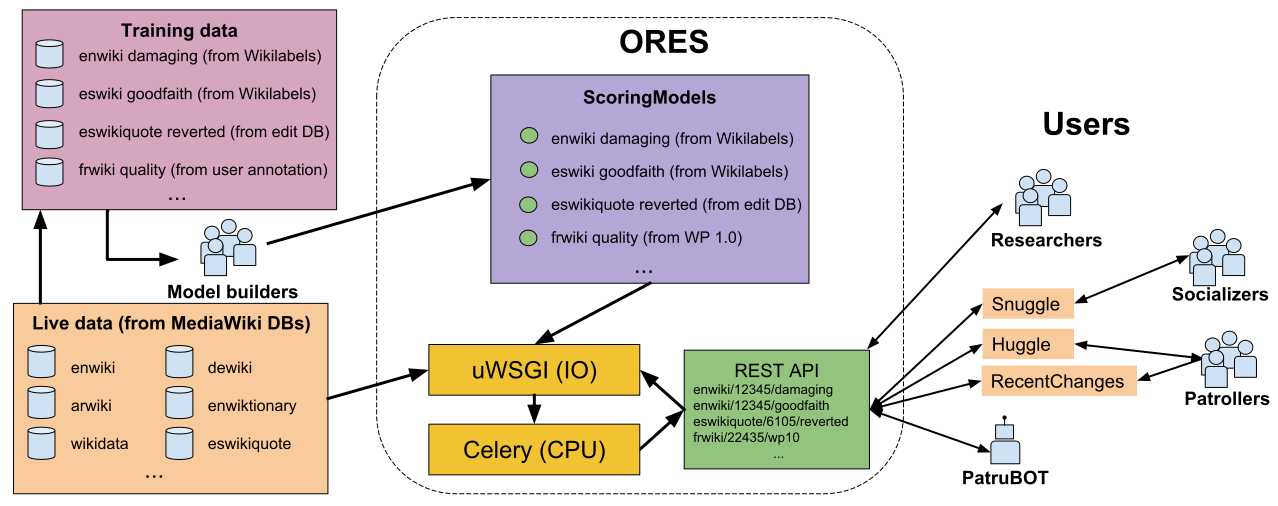
\includegraphics[width=.95\textwidth]{figures/ores_data_user_diagram}
  \caption{ORES conceptual overview.  Model builders design process for training ScoringModels from training data.  ORES hosts ScoringModels and makes them available to researchers and tool developers.}
  \label{fig:ores_data_user}
\end{figure*}

ORES has been iteratively engineered to meet the needs of Wikipedia editors and the tools that support their work (see section~\ref{sec:ores_system_engineering}). It is a machine learning as a service platform that enables Wikipedians and researchers to commission a new classifier, which are hosted by the Wikimedia Foundation for anyone to query. Figure  \ref{fig:ores_data_user} gives a conceptual overview, showing how ORES is a collection of machine classifier models and an web-based API, which connect to various sources of training data (to build the models) and live data (to apply the models). These models are designed and engineered by a varied set of model builders, some are external researchers and others are our own engineering team.  The models that ORES hosts are based on quite different sets of curated training data and have been engineered to support Wikipedian processes related to damage-detection, quality-assessment, and topic-routing. In general, the system is adaptable to a wide range of other models.

To make these models available for users, ORES implements a simple container service where the ``container,'' referred to as a \emph{ScoringModel}, represents a fully trained and tested prediction model.  All \emph{ScoringModels} contain metadata about when the model was train/tested and code for feature extraction.  All predictions take the form of a JSON document.  The ORES service provides access to ScoringModels via a RESTful HTTP interface and serves the predictions to users (see Figure~\ref{fig:english_wp10_prediction} for an example score request/response).  We chose this service structure because Wikimedian tool developers (our target audience) are familiar with this RESTful API/JSON workflow due to their common use of the MediaWiki API which employs a similar pattern.  While our target users may not have the expertise to build and maintain machine prediction models, they clearly have the expertise to make use this type of external API.

\subsection{Score documents}
\label{sec:appendix.score_documents}
The predictions made by ORES are human- and machine-readable.  In general, our classifiers will report a specific prediction along with a set of probability (likelihood) for each class.  By providing detailed information about a prediction, we allow users to re-purpose the prediction for their on use.  Consider the article quality (wp10) prediction output in Figure~\ref{fig:english_wp10_prediction}.

\begin{figure}[h!]
        \makebox{\hrulefill}{
        \small
        \begin{verbatim}
"wp10": {
  "score": {
    "prediction": "Start",
    "probability": {
      "FA": 0.00329313015, "GA": 0.0058529554,
      "B": 0.06062338048, "C": 0.01991363271,
      "Start": 0.754330134, "Stub": 0.1559867667
    }
  }
}
        \end{verbatim}
        \hrule
        \normalsize}
        \caption{A score document -- the result of \url{https://ores.wikimedia.org/v3/scores/enwiki/34234210/wp10}}
        \label{fig:english_wp10_prediction}
\end{figure}

A developer making use of a prediction like this may choose to present the raw prediction ``Start'' (one of the lower quality classes) to users or to implement some visualization of the probability distribution across predicted classed (75\% Start, 16\% Stub, etc.).  They might even choose to build an aggregate metric that weights the quality classes by their prediction weight (e.g. Ross's student support interface\cite{ross2016visualizing} or the \emph{weighted sum} metric from~\cite{halfaker2017interpolating}).

\subsection{Model information}
\label{sec:appendix.model_information}
In order to use a model effectively in practice, a user needs to know what to expect from model performance.  E.g. how often is it that when an edit is predicted to be ``damaging'' it actually is? (\emph{precision}) or what proportion of damaging edits should I expect will be caught by the model? (\emph{recall})  The target metric of an operational concern depends strongly on the intended use of the model.  Given that our goal with ORES is to allow people to experiment with the use and to appropriate prediction models in novel ways, we sought to build an general model information strategy.

\begin{figure}[htbp]
        \makebox{\hrulefill}{
        \small
        \begin{verbatim}
"damaging": {
  "type": "GradientBoosting",
  "version": "0.4.0",
  "environment": {"machine": "x86_64", ...},
  "params": {"center": true, "init": null,
             "label_weights": {"true": 10},
             "labels": [true, false],
             "learning_rate": 0.01,
             "min_samples_leaf": 1,
             ...},
  "statistics": {
    "counts": {
      "labels": {"false": 18702, "true": 743},
      "n": 19445,
      "predictions": {
        "false": {"false": 17989, "true": 713},
        "true": {"false": 331, "true": 412}}},
    "precision": {
      "labels": {"false": 0.984, "true": 0.34},
      "macro": 0.662, "micro": 0.962},
    "recall": {
      "labels": {"false": 0.962, "true": 0.555},
      "macro": 0.758, "micro": 0.948},
    "pr_auc": {
      "labels": {"false": 0.997, "true": 0.445},
      "macro": 0.721, "micro": 0.978},
    "roc_auc": {
      "labels": {"false": 0.923, "true": 0.923},
      "macro": 0.923, "micro": 0.923},
    ...
  }
}
        \end{verbatim}
        \hrule
        \normalsize}
        \caption{Model information for an English Wikipedia damage detection model -- the result of \url{https://ores.wikimedia.org/v3/scores/enwiki/?model_info&models=damaging}}
        \label{fig:english_damaging_model_info}
\end{figure}

The output captured in Figure~\ref{fig:english_damaging_model_info} shows a heavily trimmed JSON (human- and machine-readable) output of \emph{model\_info} for the ``damaging'' model in English Wikipedia.  Note that many fields have been trimmed in the interest of space with an ellipsis (``...'').  What remains gives a taste of what information is available.  Specifically, there is structured data about what kind of model is being used, how it is parameterized, the computing environment used for training, the size of the train/test set, the basic set of fitness metrics, and a version number so that secondary caches know when to invalidate old scores.  A developer using an ORES model in their tools can use these fitness metrics to make decisions about whether or not a model is appropriate and to report to users what fitness they might expect at a given confidence threshold.

\subsection{Threshold optimization}
\label{sec:appendix.threshold_optimization}
When we first started developing ORES, we realized that operational concerns of Wikipedia's curators need to be translated into confidence thresholds for the prediction models.  For example, counter-vandalism patrollers seek to catch all (or almost all) vandalism before it stays in Wikipedia for very long.  That means they have an operational concern around the \emph{recall} of a damage prediction model.  They would also like to review as few edits as possible in order to catch that vandalism.  So they have an operational concern around the \emph{filter rate}---the proportion of edits that are not flagged for review by the model\cite{halfaker2016notes}.

By finding the threshold of prediction likelihood that optimizes the filter-rate at a high level of recall, we can provide vandal-fighters with an effective trade-off for supporting their work.  We refer to these optimizations in ORES as \emph{threshold optimizations} and ORES provides information about these thresholds in a machine-readable format so that tool developers can write code that automatically detects the relevant thresholds for their wiki/model context.

Originally, when we developed ORES, we defined these threshold optimizations in our deployment configuration.  But eventually, it became apparent that our users wanted to be able to search through fitness metrics to choose thresholds that matched their own operational concerns.  Adding new optimizations and redeploying quickly became a burden on us and a delay for our users.  In response, we developed a syntax for requesting an optimization from ORES in real-time using fitness statistics from the models tests. E.g. \texttt{maximum recall @ precision >= 0.9} gets a useful threshold for a counter-vandalism bot or \texttt{maximum filter\_rate @ recall >= 0.75} gets a useful threshold for semi-automated edit review (with human judgement).

\begin{figure}[htbp]
        \makebox{\hrulefill}{
        \small
        \begin{verbatim}
  {"threshold": 0.32, ...,
   "filter_rate": 0.89, "fpr": 0.087,
   "precision": 0.23, "recall": 0.75}
        \end{verbatim}
        \hrule
        \normalsize}
        \caption{A threshold optimization -- the result of \url{https://ores.wikimedia.org/v3/scores/enwiki/?models=damaging&model_info=statistics.thresholds.true.'maximum filter_rate @ recall >= 0.75'}}
        \label{fig:english_damaging_threshold_optimization}
\end{figure}

Consider figure~\ref{fig:english_damaging_threshold_optimization}.  This result shows that, when a threshold is set on 0.299 likelihood of damaging=true, a user can expect to get a recall of 0.751, precision of 0.215, and a filter-rate of 0.88.  While the precision is low, this threshold reduces the overall workload of vandal-fighters by 88\% while still catching 75\% of (the most egregious) damaging edits.

\section{Innovations in openness}
\label{sec:innovations_in_openness}
We developed ORES in the context of Wikipedia, which generally sees itself as an egalitarian, decentralized, and radically transparent community.  With ORES, we sought to maintain these values in our system design and model building strategies.  The flow of data --- from random samples through model training, evaluation, and application --- is open for review, critique, and iteration.  We have also developed novel strategies for opening ORES models up to evaluation, experimentation, and play based on user requests.  In this section, we describe some of the key, novel innovations that have made ORES fit Wikipedian concerns and be flexible to re-appropriation.  Appendix~\ref{sec:appendix} also contains information about ORES' detailed prediction output, how users and tools can adjust their use to model fitness, and how the whole model development workflow is made inspectable and replicable.

\subsection{Collaboratively labeled data}
There are two primary strategies for gathering labeled data for training ORES' models: found traces and manual labels.

\leadin{Found traces} For many models, the MediaWiki platform records a rich set of digital traces that can be assumed to reflect a useful human judgement for modeling.  For example, in Wikipedia, it is very common that damaging edits will eventually be reverted\footnote{In Wikipedian parlance, a ``revert'' is a direct undoing of an edit, bringing the article to the exact same state it was in before.} and that good edits will not be reverted.  Thus the revert action (and remaining traces) can be used as an endogenous label in training.  We have developed a re-usable script\footnote{see \emph{autolabel} in \url{https://github.com/wiki-ai/editquality}} that when given a sample of edits, will label the edits as ``reverted\_for\_damage'' or not based on a set of constraints: the edit was reverted within 48 hours, the reverting editor was not the original editor, and the edit was not later restored by someone other than the original editor.

However, this ``reverted\_for\_damage'' label is problematic in that many edits are reverted not because they are damaging, but instead because they are tied up in an editorial dispute.  Operationalizing quality by exclusively measuring what persists in Wikipedia reinforces Wikipedia's well-known systemic biases, which is a similar problem in using found crime data in predictive policing \cite{richardson2019dirty}.  Also, the label does not differentiate damage that is a good-faith mistake from damage that is intentional vandalism.  So in the case of damage prediction models, we only make use of the ``reverted\_for\_damage'' label when manually labeled data is not available.

%\input{figures/wikilabels_screenshot}
\leadin{Manual labeling campaigns with Wiki Labels}
We hold manual labeling by human Wikipedians as the gold standard for purposes of training a model to replicate human judgement.  By asking Wikipedians to demonstrate their judgement on examples from their own wikis, we can most closely tailor model predictions to match the judgements that make sense to these communities.  This contrasts with found data, which deceptively appears to be a better option because of its apparent completeness: every edit was either reverted or not.  In contrast, manual labeling has a high up-front expense of human labor.  To minimize that cost, we developed a high-speed, collaborative labeling interface called ``Wiki Labels\footnote{\url{http://enwp.org/:m:Wiki labels}}'' to allow Wikipedians to efficiently label large datasets.

For example, to supplement our models of edit quality, we replace the models based on ``reverted\_for\_damage'' found traces with judgments from a community labeling campaign, where we specifically ask labelers to distinguish ``damaging'' edits from ``good-faith'' edits. ``Good faith'' is a well-established term in Wikipedian culture\footnote{\url{https://enwp.org/WP:AGF}}, with specific local meanings that are different than their broader colloquial use---similar to how Wikipedians define ``consensus'' or ``neutrality''.  Using these labels we can build two separate models which allow users to filter for edits that are likely to be good-faith mistakes\cite{halfaker2017automated}, to just focus on vandalism, or to apply themselves broadly to all damaging edits.

\subsection{Dependency injection and interrogability}
One of the key features of ORES that allows scores to be generated in an efficient and flexible way is a dependency injection framework.  We use a dependency solver to determine what data is necessary for a scoring job and eventually compute the features used by a prediction model.

The flexibility provided by the dependency injection framework lets us implement a novel strategy for exploring \emph{how} ORES' models make predictions.  By exposing the features extracted to ORES users and allowing them to inject their own features, we can allow users to ask how predictions would change if the world were different.  Let's say you wanted to explore how ORES judges unregistered (anon) editors differently from registered editors.  Figure~\ref{fig:anon_injection} demonstrates two prediction requests to ORES.

\begin{figure*}[h]
\centering
\begin{subfigure}[t]{.5\textwidth}
  \makebox{\hrulefill}{
  \small
  \begin{verbatim}
  "damaging": {
    "score": {
      "prediction": false,
      "probability": {
        "false": 0.938910157824447,
        "true": 0.06108984217555305   }   }  }
  \end{verbatim}
  \hrule
  \normalsize}
  \caption{Prediction with \texttt{anon = false} injected}
  \label{fig:anon_injection_false}
\end{subfigure}~~
\begin{subfigure}[t]{.5\textwidth}
  \makebox{\hrulefill}{
  \small
  \begin{verbatim}
  "damaging": {
    "score": {
      "prediction": false,
      "probability": {
        "false": 0.9124151990561908,
        "true": 0.0875848009438092   }   }   }
  \end{verbatim}
  \hrule
  \normalsize}
  \caption{Prediction with \texttt{anon = true} injected}
  \label{fig:anon_injection_true}
\end{subfigure}
\caption{Two ``damaging'' predictions about the same edit are listed for ORES.  In one case, ORES is asked to make a prediction assuming the editor is unregistered (anon) and in the other, ORES is asked to assume the editor is registered.}
\label{fig:anon_injection}
\end{figure*}

Figure~\ref{fig:anon_injection_false} shows that ORES' ``damaging'' model concludes that the edit identified by the \emph{revision ID} of 34234210 is not damaging with 93.9\% confidence.  We can ask ORES to make a prediction about the exact same edit, but to assume that the editor was unregistered (anon). Figure~\ref{fig:anon_injection_true} shows the prediction if edit were saved by an anonymous editor.  ORES would still conclude that the edit was not damaging, but with less confidence (91.2\%).  By following a pattern like this for a single edit or a set of edits, we can get to know how ORES prediction models account for anonymity through experience with practical examples. 

\subsubsection{In use}
[interrogability as a way to respond to questions about false positives]
Interrogability has also been used in creative new ways beyond bias explorations.  Some of our users have used the feature injection system to expose \emph{hypothetical} predictions to support their work.  See the discussion of Ross's work recommendation tools in Section~\ref{sec:adoption_patterns}.

\section{Adoption patterns}
\label{sec:adoption_patterns}
ORES as a socio-technical system has helped us 1) refine our understandings of volunteers' needs across wiki communities, 2) identify and address biases in ORES's models, and 3) reflect on how people think about what types of automation they find acceptable in their \emph{spaces}.  Through our open participatory process with various Wikipedian communities, we have arrived at several innovations in open machine learning practice that represent advancements in the field.

As we stated in Section~\ref{sec:design_rationale}, we measure success in new conversations about how algorithmic tools affect editing dynamics, as well as new types of tools that take advantage of these resources, implementing alternative visions of what Wikipedia is and ought to be.  We have demonstrated through discussion of adoption patterns and case studies in reflection around the use of algorithmic systems that something fundamental is \emph{working}.  ORES is being heavily adopted.  The meaning of ORES models is being re-appropriated.  Both the models and the technologies that use the models are being collaboratively audited by their users and those who are affected.

\subsection{Participatory machine learning}
In a world increasingly dominated by for-profit content platforms --- often marketed by their corporate owners as ``communities'' \cite{gillespie2018custodians} --- Wikipedia is an anomaly. While the non-profit Wikimedia Foundation has only a fraction of the resources as Facebook or Google, the unique principles and practices in the broad Wikipedia/Wikimedia movement are a generative constraint. ORES emerged out of this context, operating at the intersection of a pressing need to deploy efficient machine learning at scale for content moderation, but to do so in ways that enable volunteers to develop and deploy advanced technologies on their own terms. Our approach is in stark contrast to the norm in machine learning research and practice, which involves a more top-down mode of developing the most precise classifiers for a known ground truth, then wrap those classifiers in a complete technology for end-users, who must treat them as black boxes.

The more wiki-inspired approach to what we call ``participatory machine learning'' imagines classifiers to be just as provisional and open to skeptical reinterpretation as the content of Wikipedia's encyclopedia articles. And like Wikipedia articles, we suspect some classifiers will be far better than others based on how volunteers develop and curate them, for various definitions of ``better'' that are already being actively debated. Our case studies briefly indicate how volunteers have collectively engaged in sophisticated discussions about how they ought to use machine learning. ORES' fully open, reproducible, and audit-able code and data pipeline---from training data to models to scored predictions---enables a wide range of new collaborative practices. ORES is a more socio-technical and CSCW-oriented approach to issues in the FATML space, where attention is often placed on technical solutions, like interactive visualizations for model interpretability or mathematical guarantees of operationalized definitions of fairness.  Our approach is specific to the particular practices and values of Wikipedia, and we have shown how ORES has been developed to fit into this context.

ORES also represents an innovation in openness in that it decouples several activities that have typically all been performed by engineers or under their direct supervision: choosing or curating training data, building models to serve predictions, auditing predictions for false positives/negatives, and developing interfaces or automated agents that act on those predictions. Often, those who develop and maintain the technical infrastructure for systems gain what we can call an \textit{incidental jurisdiction} over the other areas, which does not necessarily require that same expertise. As our cases have shown, people with extensive contextual and domain expertise in an area can make well-informed decisions about curating training data, identifying false positives/negatives, setting thresholds, and designing interfaces that use scores from a classifier. In decoupling these actions, ORES helps delegate these responsibilities more broadly, opening up the structure of the socio-technical system and expanding who can participate in it.

\subsection{Critical reflection}
In section~\ref{sec:case_studies}, we showed evidence of critical reflection on the current processes and the role of algorithms in quality control.  These case studies show that collaborative auditing is taking place, that there is a proliferation of tools based on alternative uses of ORES we did not imagine, and that that Wikipedians have more agency over their quality control processes. We also see an important expansion into supporting non-English language Wikipedias, which have historically not received as much support in this area. We are inspired by much of the concern that has surfaced for looking into biases in ORES' prediction models (e.g. anon bias and the Italian ``ha'') and over what role algorithms should have in directly reverting human actions (e.g. PatruBOT and Dexbot).

Eliciting this type of critical reflection and empowering users to engage in their own choices about the roles of algorithmic systems in their social spaces has typically been more of a focus from the Critical Algorithms Studies literature, which comes from a more humanistic and interpretivist social science perspective (e.g. \cite{barocas2013governing, kitchin2017thinking}. This literature also emphasizes a need to see algorithmic systems as dynamic and constantly under revision by developers \cite{seaver2017algorithms} --- work that is invisible in most platforms, but is foregrounded in ORES. In these case studies, we see that given ORES' open API and Wikipedia's collaborative wiki pages, Wikipedians will audit ORES' predictions and collaborate with each other to build information about trends in ORES' mistakes and how they expected their own processes to function.

\subsection{Design implications}
In many user-generated content communities (UGCs), the technologies that mediate social spaces are technically controlled by a single organization. Much work in exploring fairness in machine learning advocates decentralized services, but we have shown how if such an organization seeks to involve its users and stakeholders in the process, they can employ a \emph{decoupling} strategy like that of ORES, where the infrastructural expertise needed to build and serve ML models at scale is managed by the professionals, while other stakeholders curate training data, audit model performance, and decide where and how the ML models will be used. The case studies show the feasibility and benefits of decoupling the ML modeling service from the curation of training data and the implementation of ML scores in interfaces and tools, as well as in moving away from a single ``one classifier to rule them all'' and towards giving users the ability to train and serve models. 

We show how with such a service, non-technical users can and do play critical roles in the governance of ML in Wikipedia, which go beyond what they would be capable of if ORES were simply another ML classifier hidden behind a single-purpose UI albeit with open-source code and training data (which is what prior ML models in Wikipedia were). Because ORES is a service in production designed to let others more easily train and deploy their own models, this achieves a critical decoupling between algorithmic prediction and the intended use -- thus encouraging and enabling re-appropriation.  This strategy reduces incidental complexities involved in developing the systems necessary for deploying ML in production and at scale and turns that ML into a common resource on which others can audit and make use of separately from any specific implementation.

Specifically, our design implications for UGCs is to take this literally: to run open ML as a service platforms so that users can build their own models with training datasets they provide, which serve predictions using open APIs, and support activities like \emph{feature injection} and \emph{threshold optimization} for auditing and re-appropriation. Together with a common set of discussion spaces like the ones Wikipedians used, these can enable the re-use of models by a broader audience and encourage/make space for reflective practices such as model auditing, decision-making about thresholds, or the choice between different classifiers trained on different training datasets.  Our work shows that that non-technical users (at least in our field site) have an interest in participating in such governance activities and that such users can effectively coordinate common understandings of what a machine learning model is doing and whether or not that is acceptable to them.

\subsection{Future work}
Observing ORES in practice suggests avenues of future work toward crowd-based auditing tools.  As our case studies suggest, auditing of ORES' predictions and mistakes has become a popular activity.  Even though we did not design interfaces for discussion and auditing, some Wikipedians have used unintended affordances of wiki pages and MediaWiki's template system to organize processes for flagging false positives and calling them to our attention.  This process has proved invaluable for improving model fitness and addressing critical issues of bias against disempowered contributors.  To better facilitate this process, future system builders should implement structured means to refute, support, discuss, and critique the predictions of machine models.  With a structured way to report what machine prediction gets right and wrong, we can make it easier for tools that use ORES to also allow for reporting mistakes and for others to infer trends.  For example, a database of ORES mistakes could be queried in order to build the kind of thematic analyses that Italian Wikipedians showed us (see section~\ref{sec:case_studies}).  By supporting such an activity, we are working to transfer more power from ourselves and to our users.  Should one of our models develop a nasty bias, our users will be more empowered to coordinate with each other, show that the bias exists and where it causes problems, and either get the model's predictions turned off or even shut down the use of ORES (e.g. PatruBOT).

We also look forward to what those from fairness in MN and critical algorithm studies can do with ORES, which is far more open than most high-scale machine learning applications. Most of the studies and critiques of \emph{subjective algorithms}\cite{tufekci2015algorithms} focus on for-profit organizations that are strongly resistant to external interrogation. Wikipedia is one of the largest and arguably most impactful information resources in the world, and decisions about what is and is not represented have impacts across all sectors of society.  The algorithms that ORES makes available are part of the decision process that leads to some people's contributions remaining and others being removed.  This is a context where \emph{algorithms matter to humanity}, and we are openly experimenting with the kind of transparent and open processes that \emph{fairness and transparency in machine learning} researchers are advocating.  Yet, we have new problems and new opportunities.  There is a large body of work exploring how biases manifest and how unfairness can play out in algorithmically mediated social contexts.  ORES would be an excellent place to expand the literature within a specific and important field site.

Finally, we also see potential in allowing Wikipedians to freely train, test, and use their own prediction models without our engineering team involved in the process.  Currently, ORES is only suited to deploy models that are trained and tested by someone with a strong modeling and programming background, and we currently do that work for those who come to us with a training dataset and ideas about what kind of classifier they want to build.  That does not necessarily need to be the case.  We have been experimenting with demonstrating ORES model building processes using Jupyter Notebooks\footnote{\url{http://jupyter.org}} \footnote{e.g. \url{ https://github.com/wiki-ai/editquality/blob/master/ipython/reverted_detection_demo.ipynb}} and have found that new programmers can understand the work involved.  This is still not the holy grail of crowd-developed machine prediction, where all of the incidental complexities involved in programming are removed from the process of model development and evaluation.  Future work exploring strategies for allowing end-users to build models that are deployed by ORES would surface the relevant HCI issues involved and the changes to the technological conversations that such a margin-opening intervention might provide.


\section{Case studies in reflection}
\label{sec:case_studies}
\input{sections/7_conclusion}

\section{Acknowledgements}
\label{sec:acknowledgements}
REDACTED FOR REVIEW


\section{Appendix}
See the supplementary material for the Appendix section.

% Bibliography
\bibliographystyle{ACM-Reference-Format}
\bibliography{refs}

\pagebreak
\appendix
\section{Appendix}
\label{sec:appendix}
\subsection{ORES system details}
In this section, we describe some of the details of the ORES system.

\subsubsection{Score documents}
\label{sec:appendix.score_documents}
The predictions made by through ORES are human- and machine-readable.  In general, our classifiers will report a specific prediction along with a set of probability (likelihood) for each class.  By providing detailed information about a prediction, we allow users to re-purpose the prediction for their on use.  Consider article quality (wp10) prediction output in Figure~\ref{fig:english_damaging_model_info}.

\begin{figure}[htbp]
        \makebox{\hrulefill}{
        \small
        \begin{verbatim}
        "wp10": {
          "score": {
            "prediction": "Start",
            "probability": {
              "FA": 0.0032931301528326693, "GA": 0.005852955431273448,
              "B": 0.060623380484537165, "C": 0.01991363271632328,
              "Start": 0.7543301344435299, "Stub": 0.15598676677150375
            }
          }
        }
        \end{verbatim}
        \hrule
        \normalsize}
        \caption{Result of \url{https://ores.wikimedia.org/v3/scores/enwiki/34234210/wp10}}
        \label{fig:english_damaging_model_info}
\end{figure}

A developer making use of a prediction like this may choose to present the raw prediction ``Start'' (one of the lower quality classes) to users or to implement some visualization of the probability distribution across predicted classed (75\% Start, 16\% Stub, etc.).  They might even choose to build an aggregate metric that weights the quality classes by their prediction weight (e.g. Ross's student support interface\cite{ross2016visualizing} or the \emph{weighted sum} metric from \cite{halfaker2017interpolating}).

\subsubsection{Model information}
\label{sec:appendix.model_information}
In order to use a model effectively in practice, a user needs to know what to expect from model performance.  E.g. how often is it that when an edit is predicted to be ``damaging'' it actually is? (\emph{precision}) or what proportion of damaging edits should I expect will be caught by the model? (\emph{recall})  The target metric of an operational concern depends strongly on the intended use of the model.  Given that our goal with ORES is to allow people to experiment with the use and reflection of prediction models in novel ways, we sought to build an general model information strategy.

\begin{figure}[htbp]
        \makebox{\hrulefill}{
        \small
        \begin{verbatim}
      "damaging": {
        "type": "GradientBoosting",
        "version": "0.4.0",
        "environment": {"machine": "x86_64", ...},
        "params": {center": true, "init": null, "label_weights": {"true": 10},
                   "labels": [true, false], "learning_rate": 0.01, "min_samples_leaf": 1,
                   ...},
        "statistics": {
          "counts": {"labels": {"false": 18702, "true": 743},
                     "n": 19445,
                     "predictions": {"false": {"false": 17989, "true": 713},
                                     "true": {"false": 331, "true": 412}}},
          "precision": {"labels": {"false": 0.984, "true": 0.34},
                        "macro": 0.662, "micro": 0.962},
          "recall": {"labels": {"false": 0.962, "true": 0.555},
                     "macro": 0.758, "micro": 0.948},
          "pr_auc": {"labels": {"false": 0.997, "true": 0.445},
                     "macro": 0.721, "micro": 0.978},
          "roc_auc": {"labels": {"false": 0.923, "true": 0.923},
                      "macro": 0.923, "micro": 0.923},
          ...
        }
      }
        \end{verbatim}
        \hrule
        \normalsize}
        \caption{Result of \url{https://ores.wikimedia.org/v3/scores/enwiki/?model_info&models=damaging}}
        \label{fig:english_damaging_model_info}
\end{figure}

The output captured in Figure~\ref{fig:english_damaging_model_info} shows a heavily trimmed JSON (human- and machine-readable) output of \emph{model\_info} for the ``damaging'' model in English Wikipedia.  Note that many fields have been trimmed in the interest of space with an ellipsis (``...'').  What remains gives a taste of what information is available.  Specifically, there is structured data about what kind of model is being used, how it is parameterized, the computing environment used for training, the size of the train/test set, the basic set of fitness metrics, and a version number so that secondary caches know when to invalidate old scores.  A developer using an ORES model in their tools can use these fitness metrics to make decisions about whether or not a model is appropriate and to report to users what fitness they might expect at a given confidence threshold.

\subsubsection{Explicit pipelines}
\label{sec:appendix.explicit_pipelines}
We have designed the process of training and deploying ORES prediction models is to be repeatable and reviewable.  Consider the following code that represents a common pattern from our model-building Makefiles:
\begin{figure}[htbp]
        \makebox{\hrulefill}{
        \small
        \begin{verbatim}
datasets/enwiki.human_labeled_revisions.20k_2015.json:
        ./utility fetch_labels \
                https://labels.wmflabs.org/campaigns/enwiki/4/ > $@

datasets/enwiki.labeled_revisions.w_cache.20k_2015.json: \
                datasets/enwiki.labeled_revisions.20k_2015.json
        cat $< | \
        revscoring extract \
                editquality.feature_lists.enwiki.damaging \
                --host https://en.wikipedia.org \
                --extractor $(max_extractors) \
                --verbose > $@

models/enwiki.damaging.gradient_boosting.model: \
                datasets/enwiki.labeled_revisions.w_cache.20k_2015.json
        cat $^ | \
        revscoring cv_train \
                revscoring.scoring.models.GradientBoosting \
                editquality.feature_lists.enwiki.damaging \
                damaging \
                --version=$(damaging_major_minor).0 \
                (... model parameters ...)
                --center --scale > $@
        \end{verbatim}
        \hrule
        \normalsize}
        \caption{Makefile rules for the English damage detection model from \url{https://github.com/wiki-ai/editquality}}
        \label{fig:english_damaging_makefile}
\end{figure}


Essentially, this code helps someone determine where the labeled data comes from (manually labeled via the Wiki Labels system).  It makes it clear how features are extracted (using the \texttt{revscoring extract} utility and the \texttt{feature\_lists.enwiki.damaging} feature set).  Finally, this dataset of extracted features is used to cross-validate and train a model predicting the ``damaging'' label and a serialized version of that model is written to a file.  A user could clone this repository, install the set of requirements, and run \texttt{make enwiki\_models} and expect that all of the data-pipeline would be reproduced, and an exactly equivalent model obtained.

By explicitly using public resources and releasing our utilities and Makefile source code under an open license (MIT), we have essential implemented a turn-key process for replicating our model building and evaluation pipeline.  A developer can review this pipeline for issues knowing that they are not missing a step of the process because all steps are captured in the Makefile.  They can also build on the process (e.g. add new features) incrementally and restart the pipeline.  In our own experience, this explicit pipeline is extremely useful for identifying the origin of our own model building bugs and for making incremental improvements to ORES' models.

At the very base of our Makefile, a user can run \texttt{make models} to rebuild all of the models of a certain type.  We regularly perform this process ourselves to ensure that the Makefile is an accurate representation of the data flow pipeline.  Performing complete rebuild is essential when a breaking change is made to one of our libraries.  The resulting serialized models are saved to the source code repository so that a developer can review the history of any specific model and even experiment with generating scores using old model versions.



\end{document}
